\documentclass{beamer}

\usepackage{beamerthemeHannover,graphics,amsmath,bm}

\title[Measurement Invariance]{Generalized Measurement Invariance
  Tests for Factor Analysis}
\author{Ed Merkle\inst{1} \and Achim Zeileis\inst{2}}
\institute{\inst{1} University of Missouri \and \inst{2} Universit\"{a}t Innsbruck}
\date{Supported by grant SES-1061334 from the U.S.\ National
  Science Foundation}

\begin{document}

\frame{\titlepage}

\frame{
  \frametitle{}
  \tableofcontents}


\section{Background}
% Define measurement invariance
\frame{
  \frametitle{Measurement Invariance}
  \begin{itemize}
    \item Measurement invariance: Sets of tests/items consistently
      assigning scores across diverse groups of individuals.\\ \ \\
    \item Notable violations of measurement invariance:
      \begin{itemize}
        \item SAT for different ethnic groups (Atkinson, 2001)
        \item Intelligence tests \& the Flynn effect
          (Wicherts et al., 2004)
      \end{itemize}
  \end{itemize}}

% FA path diagram, types of MI
\frame{
  \frametitle{Example (Age $\leq$ 16)}
  % path diagram illustrating parameters being the same for everyone
  \begin{center}
      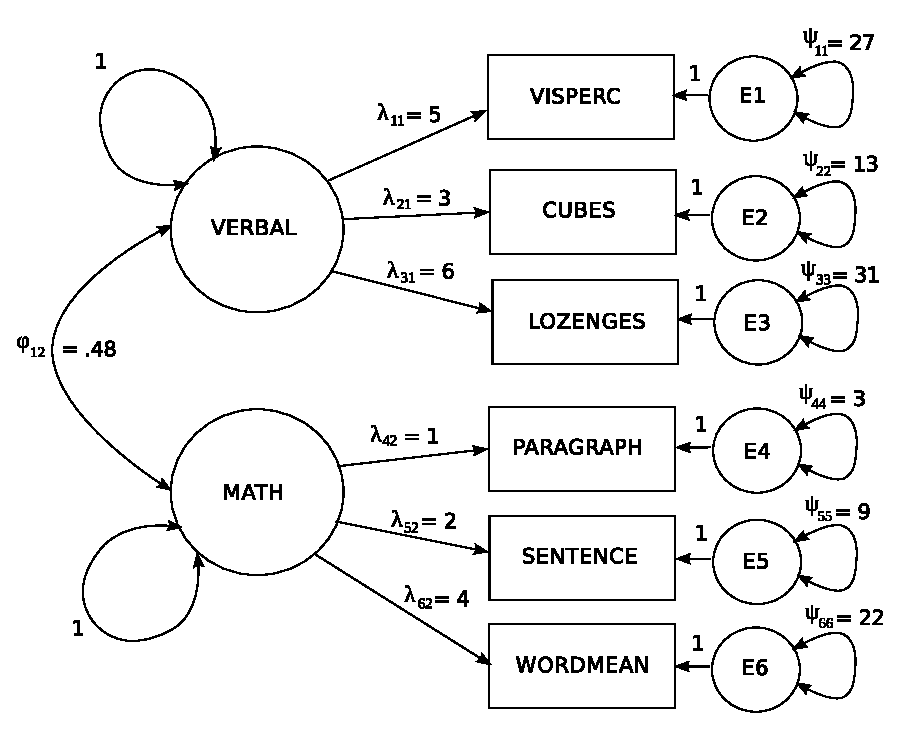
\includegraphics[height=3in]{model_under16.pdf}
  \end{center}}

\frame{
  \frametitle{Example (Age~$>$~16)}
  % path diagram illustrating parameters being the same for everyone
  \begin{center}
      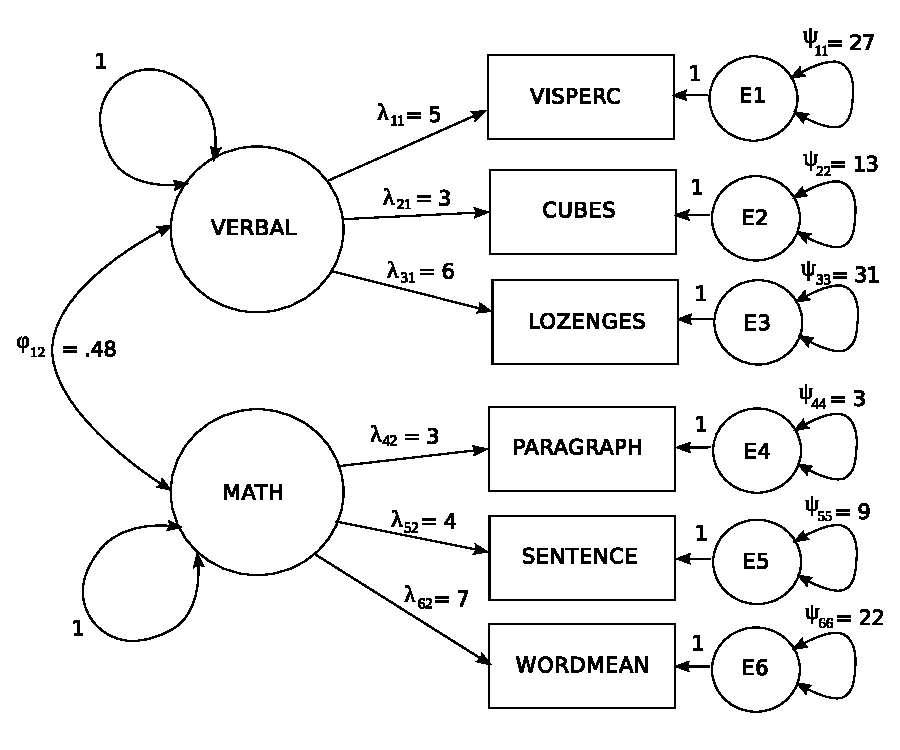
\includegraphics[height=3in]{model_over16.pdf}
  \end{center}}

% Define as theta_i = theta_0, i=1,..,n
\frame{
  \frametitle{Hypotheses}
  \begin{itemize}
    % \item There exist many types of measurement invariance,
    %   based on specific subsets of parameters being allowed
    %   to vary across individuals (e.g., Meredith, 1993).\\ \ \\
    \item Hypothesis of ``full'' measurement invariance:\\
      \begin{center}
          $H_0: \bm{\theta}_i = \bm{\theta}_0, i=1,\ldots,n$\\
          $H_1: \text{Not all the }\bm{\theta}_i = \bm{\theta}_0$
      \end{center}
      where $\bm{\theta}_i = (\lambda_{i, 1, 1}, \dots, \psi_{i, 1, 1}, \dots, \varphi_{i, 1, 2}, \dots)^\top$
      is the full $p$-dimensional parameter vector for individual $i$.
  \end{itemize}}

% Too difficult to assess, so use an auxiliary variable to place
% people in meaningful groups
  % continuous vs categorical auxiliary variable
\frame{
  \frametitle{Hypotheses}
  \begin{itemize}
    \item $H_0$ from the previous slide is difficult to fully assess
      due to all the ways by which individuals may differ.\\ \ \\
    \item We typically place people into groups based on a meaningful
      auxiliary variable, then study measurement invariance across
      those groups (via Likelihood Ratio tests, Lagrange multiplier
      tests, Wald tests).\\ \ \\
    \item If we did not know the groups in advance, we could conduct
      a LR or LM test for each possible grouping, then take the maximum.
      Requires different critical values! (Can be obtained from proposed
      tests.)
  \end{itemize}}

\frame{
  \frametitle{Lack of Grouping}
  \begin{center}
      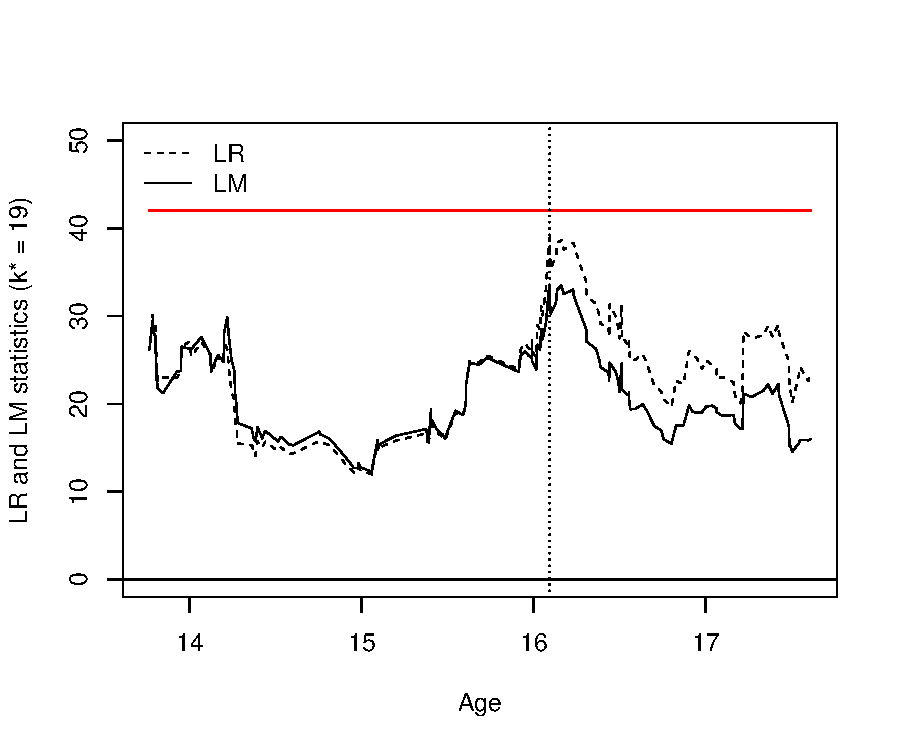
\includegraphics[height=3in]{paper-lm-lr-19.pdf}
  \end{center}
}

\section{Proposed Tests}
\frame{
  \frametitle{Proposed Tests}
  \begin{itemize}
    \item In contrast to existing tests of measurement invariance, the
      proposed tests offer the abilities to:
      \begin{itemize}
        \item Test for measurement invariance when groups are
          ill-defined (e.g., when the grouping variable is continuous).
        \item Test for measurement invariance in any subset of model
          parameters.
        \item Interpret the nature of measurement invariance violations.
      \end{itemize}
  \end{itemize}}

\frame{
  \frametitle{Proposed Tests}
  \begin{itemize}
    \item The proposed family of tests rely on first derivatives of
      the model's log-likelihood function.
    \item We can also consider individual terms ({\em scores}) of the gradient.  These scores tell us how well a particular parameter describes a particular individual.
  % Equation of gradient vs scores for individuals
  \end{itemize}
\begin{eqnarray*}
  \displaystyle\sum_{i=1}^{n} s(\hat{\bm{\theta}} ; \bm{x}_i) =
  {\bm 0},\text{ where} \\
 \\
  s(\hat{{\bm \theta}}; \bm{x}_i) = \frac{\partial}{\partial \bm{\theta}} \log
\text{L}({\bm{x}}_i, {\bm{\theta}}) \big |_{\bm{\theta} = \widehat{\bm{\theta}}}
\end{eqnarray*}}

% \frame{
%   \frametitle{Proposed Tests}
%   \begin{itemize}
%     \item We can also consider individual terms ({\em{scores}}) of the
%       gradient.  These scores tell us how well a particular
%       parameter describes a particular individual.  If your score is
%       0 for some parameter, that parameter describes you well.  If your score
%       is far from 0, that parameter describes you poorly. \\ \ \\
%   \end{itemize}
%   \begin{equation*}
%   \psi(\bm{x}_i, {\bm \theta}) = \frac{\partial}{\partial \bm{\theta}} \log
%   \text{L}({\bm{x}}_i, {\bm{\theta}}) \big |_{\bm{\theta} = \widehat{\bm{\theta}}}      
%   \end{equation*}}

\frame{
  \frametitle{Proposed Tests}
  \begin{itemize}
    \item Under measurement invariance, parameter estimates should
      roughly describe everyone equally well.  So people's scores
      should fluctuate around zero.\\ \ \\
    \item If measurement invariance is violated, the scores should
      stray from zero.
  \end{itemize}}

\begin{frame}[fragile]
  \frametitle{Aggregating Scores}
 % define cumulative scores and other notation
  \begin{itemize}
    \item We need a way to aggregate scores across people so that we
      can draw some general conclusions.
      \begin{itemize}
        \item Order individuals by an auxiliary variable.\\ \ \\
        \item Define $t \in (1/n, n)$.
          The {\em empirical cumulative score process} is defined by:\\
  \begin{equation*}
    \bm{B}(\hat{\bm{\theta}}; t) = \frac{1}{\sqrt{n}}
    \displaystyle\sum_{i=1}^{\lfloor nt 
      \rfloor} s(\hat{\bm{\theta}} ; \bm{x}_i).
    \end{equation*}
  where $\lfloor nt \rfloor$ is the integer part of $nt$.
      \end{itemize}
  \end{itemize}
\end{frame}

% EXAMPLE OF CUMULATIVE SCORE
% \frame{
%   \frametitle{Cumulative Scores}
% \begin{center}
% \begin{tabular}{rrrr}
%   \hline
%  & Age & Score & Cumul Sc \\ 
%   \hline
% 1 & 13.0 & -0.24 & -0.24 \\ 
%   2 & 13.5 & 0.17 & -0.08 \\ 
%   3 & 14.0 & -0.38 & -0.45 \\ 
%   4 & 14.5 & 0.27 & -0.19 \\ 
%   5 & 15.0 & -0.27 & -0.46 \\ 
%    \hline
% \end{tabular}
% \end{center}}

\begin{frame}[fragile]
  \frametitle{Tests}
 % show that cumulative scores follow a Brownian bridge under H_0
  \begin{itemize}
    \item Theorem: Under the hypothesis of
      measurement invariance, a functional central limit
      theorem holds:
  \begin{equation*}
  {\bm{I}}(\widehat{{\bm{\theta}}})^{-1/2}{\bm{B}}(\widehat{{\bm{\theta}}}; \cdot) 
\overset{d}{\rightarrow} {\bm B}^{0}(\cdot),
  \end{equation*}
 where ${\bm{I}}(\widehat{{\bm{\theta}}})$ is the observed
 information matrix and ${\bm B}^{0}(\cdot)$ is a
 $p$-dimensional Brownian bridge.\\ \ \\

   \item Testing procedure: Compute an aggregated statistic of empirical
     score process and compare with corresponding quantile of aggregated
     Brownian motion.\\ \ \\

    \item Test statistics: Special cases include double maximum (DM), Cram\'er-von Mises
      (CvM), maximum of LM statistics.
  \end{itemize}
\end{frame}

\frame{
  \frametitle{Simulation}
  \begin{itemize}
    \item Simulation: What is the power of the proposed tests?\\ \ \\
      \begin{itemize}
        \item Two-factor model, with three indicators each.
        \item Measurement invariance violation in three factor loading parameters, with magnitude from 0--4 standard errors.
        \item Sample size in $\{100, 200, 500\}$.
        \item Model parameters tested in $\{3, 19\}$.
        \item Three test statistics.
      \end{itemize}
  \end{itemize}}

\frame{
  \frametitle{Simulation}
  \begin{center}
      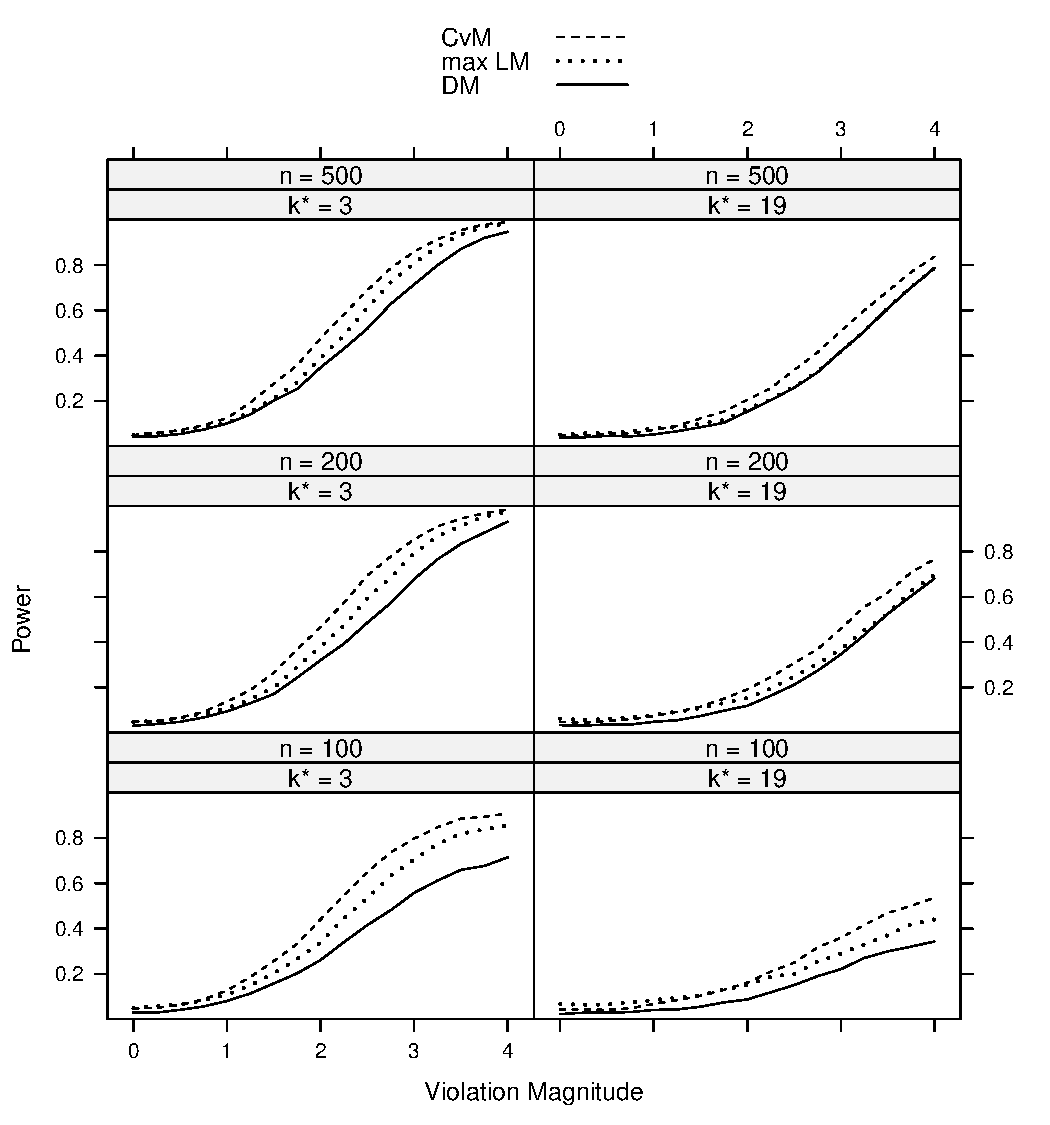
\includegraphics[height=3in]{paper-mzsim-xyplot.pdf}
  \end{center}
}

% \frame{
%   \frametitle{Brownian Bridge}
%   \begin{itemize}
%     \item Brownian bridge: A sequence of normal random variables
%       $X(t)$ satisfying:
%     % notation
% \begin{eqnarray*}
%     \mu(t) & = & 0\ \forall\ t\\
%     \Gamma(t_1, t_2) & = & \text{min}(t_1, t_2)\\
%     X(0) = & X(1) & = 0.
% \end{eqnarray*}
%   \end{itemize}}

% Picture of Brownian bridge
% \frame{
%   \frametitle{Brownian Bridge}
%   \begin{center}
%       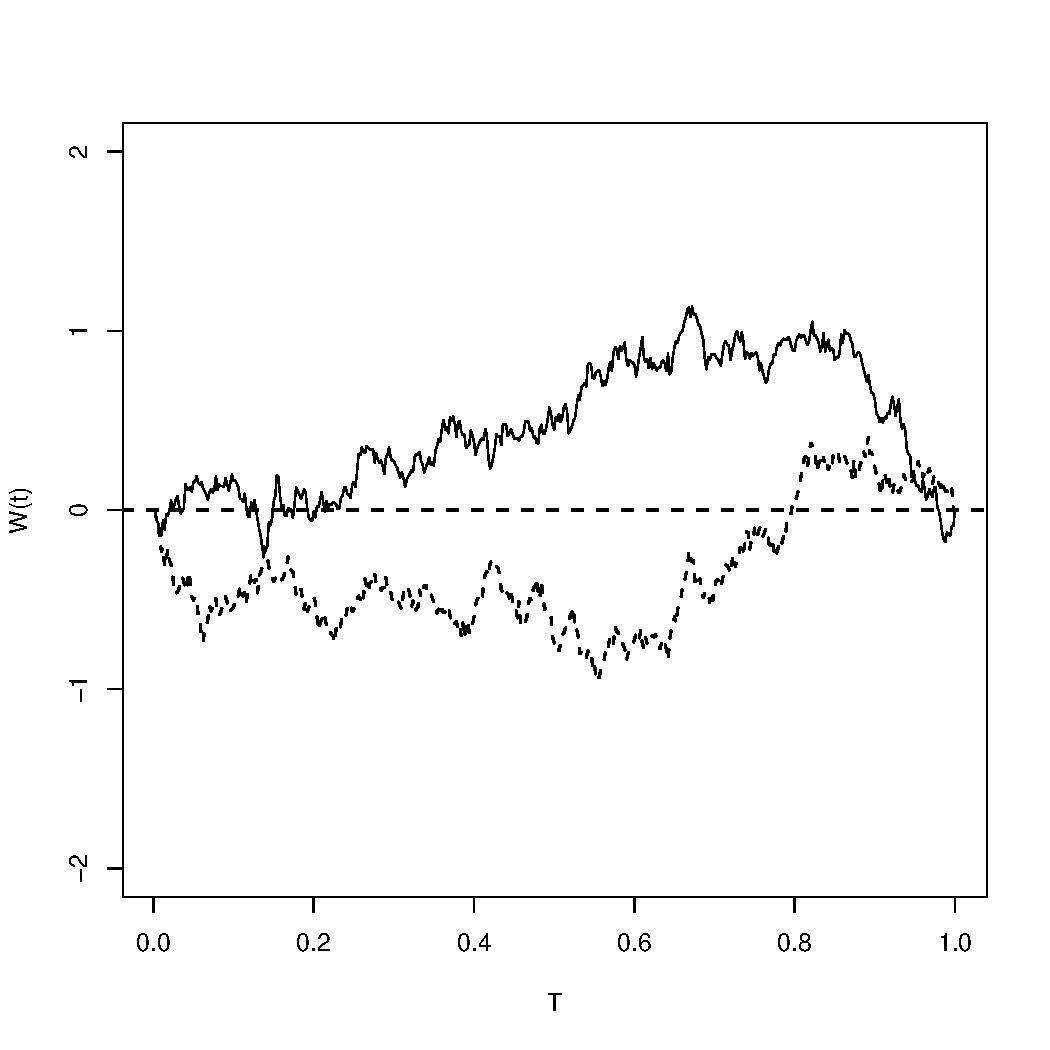
\includegraphics[height=3in]{brownian.pdf}
%   \end{center}}

% \frame{
%   \frametitle{Theorem}
%   \begin{itemize}
%     \item Use of the theorem:
%       \begin{itemize}
%         \item The theorem gives us a way to construct statistical
%           tests of measurement invariance using the scores.
%         \item Various test statistics can be obtained depending on our
%           goals.
%         \item Ordering individuals based on an auxiliary variable
%           allows us to interpret measurement invariance violations in
%           the context of that variable.
%       \end{itemize}
%   \end{itemize}}



% INSERT WICHERTS EXAMPLE HERE
\section{Illustration}
\frame{
  \frametitle{Example}
  \begin{itemize}
    \item Example: Studying stereotype threat via factor analysis (Wicherts et al., 2005)
      \begin{itemize}
        \item Stereotype threat: Knowledge of stereotypes about one's social group might cause one to fulfill the stereotypes.
        \item Wicherts et al.\ study: 295 students were administered three intelligence tests.  Stereotypes were primed for half of the students.
        \item Groups defined by: Ethnicity (majority/minority) and whether or not stereotypes were primed.
      \end{itemize}
  \end{itemize}}

\frame{
  \frametitle{Model}
  \begin{itemize}
    \item To study the data, Wicherts et al.\ employed a series of four-group, one-factor models.
      \begin{itemize}
        \item General finding: Minorities with stereotype primes have different measurement parameters than other groups.
        \item Current example: Is measurement further impacted by academic performance (as measured by student GPA)?
      \end{itemize}
  \end{itemize}}

\frame{
  \frametitle{Model}
  \begin{itemize}
    \item We utilize a model employed by Wicherts et al., where four model parameters are specific to the ``minority, stereotype prime'' group.
      \begin{itemize}
        \item Test for measurement invariance in these parameters wrt the student GPA variable (either all four together or only the factor mean).
        \item Violations of measurement invariance imply that stereotype threat is more problematic for students of low or high GPA.
      \end{itemize}
  \end{itemize}}

\frame{
  \frametitle{Results for Single Parameters}
  \begin{center}
      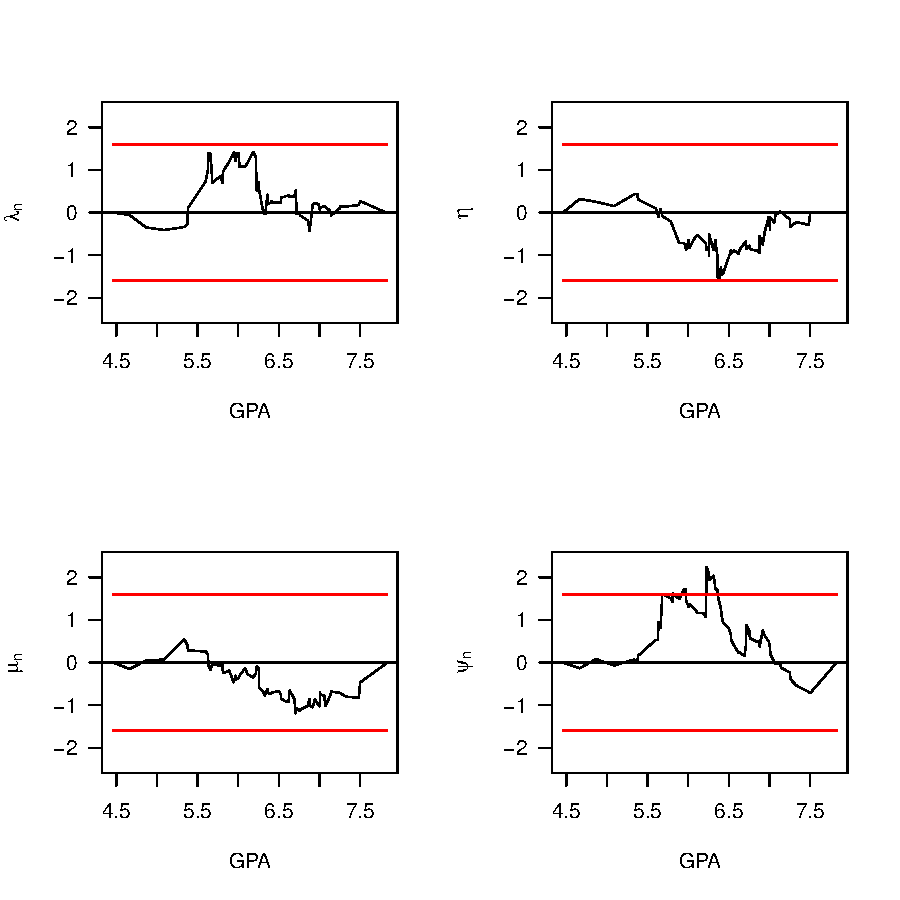
\includegraphics[height=3in]{gefp_4_ind.pdf}
  \end{center}}

\frame{
  \frametitle{Aggregated Results}
  \begin{center}
      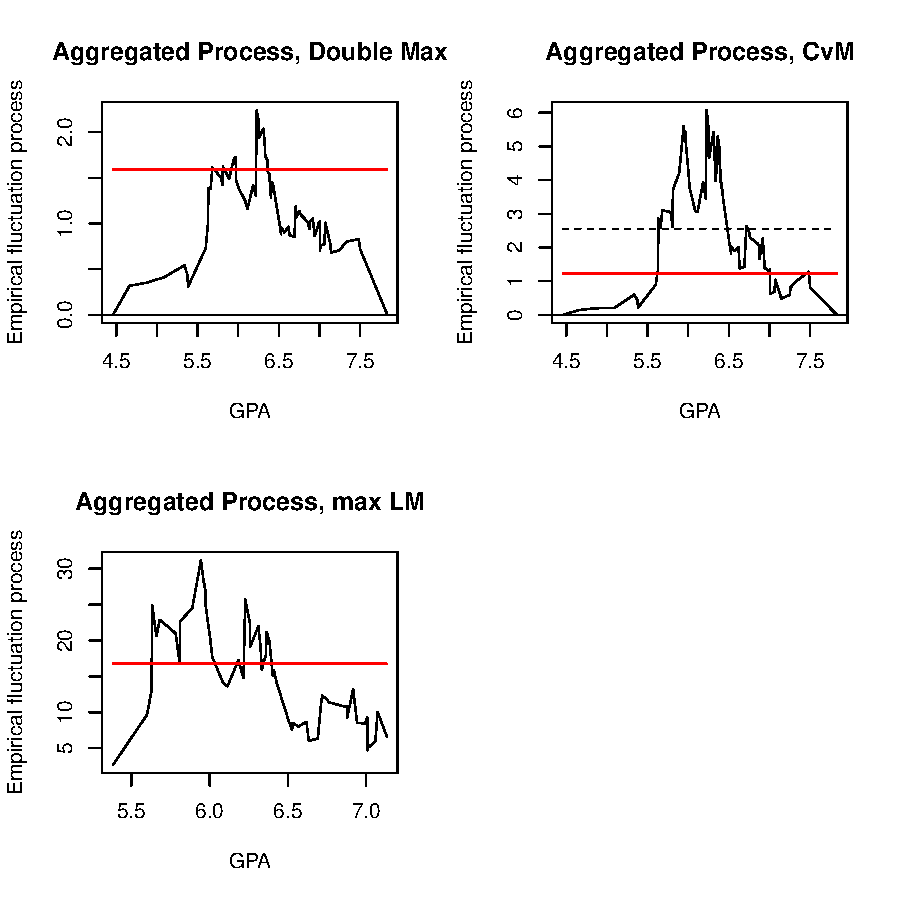
\includegraphics[height=3in]{gefp_4_agg.pdf}
  \end{center}}

\section{Conclusions}
\frame{
  \frametitle{Conclusions}
  \begin{itemize}
    \item Measurement invariance tests utilizing stochastic processes have 
      important advantages over existing tests:
      \begin{itemize}
        \item Isolating specific parameters that violate
          measurement invariance, allowing the researcher to define
          specific types of measurement invariance ``post hoc''
          instead of ``a priori''.
        \item Isolating
          groups of individuals whose parameter values differ.
        \item Studying the impact of continuous variables on model estimates, without ``ruining'' the rest of the model.
      \end{itemize}
    \item Power is reasonable, with specific tests being better in
      specific circumstances.
  \end{itemize}}

\frame{
  \frametitle{Software}
  \begin{itemize}
    \item To carry out the tests, we utilize
      \begin{itemize}
        \item \texttt{lavaan} for model estimation.
        \item \texttt{estfun()} for score extraction, which is currently a combination of our own code and \texttt{lavaan} code.
        \item \texttt{strucchange} for carrying out the proposed tests with the scores.
          \begin{itemize}
            \item Required input: Fitted model, function for score extraction, and information matrix (optional).
            \item \texttt{gefp()} constructs the process.
            \item \texttt{sctest()} and \texttt{plot()} calculate and visualize test statistics.
          \end{itemize}
      \end{itemize}
  \end{itemize}}


\frame{
  \frametitle{Current Work}
  \begin{itemize}
    \item Continued test implementation via \texttt{strucchange} and \texttt{lavaan} (and possibly \texttt{OpenMx}).\\ \ \\
    \item Detailed examination of test properties via simulation.\\ \ \\
    \item Extension to related psychometric issues.\\ \ \\
    \item Working paper: \url{http://econpapers.repec.org/RePEc:inn:wpaper:2011-09}
  \end{itemize}}

\frame{
  \frametitle{}
  \begin{itemize}
  \item Questions?
  \end{itemize}}

\end{document}
